\section{Problemanalyse}\todo{Mangler vi ikke en overgang/ indledning mellem Internet of Things og Problemanalyse?}

    I nyhederne har der været historier om firmaer som Dahua, hvor sikkerheden på IoT enheder bliver nedprioriteret for at maksimere den mulige indtjening. I situationen med firmaet Dahua, blev deres IoT kameraer hacket og brugt til et \Gls{DDoS_angreb} mod DNS udbyderen Dyn \autocite{MotherboardVice}. Dette fik flere hjemmesider såsom Twitter, Spotify og Reddit til at lukke ned. \\ 
    Herefter blev Dahua tvunget til at lukke de sikkerhedshuller som mange siger var pinligt nemme at fikse. Med en skandale som dette kan man se en af de mange muligheder hvorpå svagt sikrede IoT enheder kan anvendes af ondsindede hackere til egne formål. Dahua er dog langt fra den eneste IoT udbyder som har nedprioriteret sikkerhedsaspekterne vedrørende deres enheder, for at få en økonomisk fordel i forhold til deres konkurrenter. En økonomisk tilgang til IoT som dette medføre et marked fyldt med enheder, som ikke har brugerens sikkerhed i mente. De enheder hvor sikkerheden ikke bliver prioriteret, udgør en nemmere vej til at få adgang til et LAN (Local Area Network) og dets enheder, og bruge informationerne til ondsindede formål.  
    
    \autocite{Androidauthority}\\
    Som sagt ligger problemet med IoT enheder ofte i at der ikke bliver gjort meget ud af sikkerhedsaspekterne. Der skal foreksempel implementeres nogle sikkerhedsforanstaltninger som bliver sat som krav for alle firmaer som står for produktionen af IoT enheder.\\ 
    Det samme burde gælde for firmaer som Dahuas og deres IoT enheder. 
    Her kan der tales om noget så nemt som at sikre sig at de samme brugernavne og koder ikke bliver brugt til de samme IoT enheder. Det kræver kun en simpel Google søgning for at finde koderne online. Koder og brugernavne skal være unikke og stærke for at optimere sikkerheden. Disse skal herefter klistr es på den enkelte IoT enhed, så det kun er ejeren af IoT enheden der kan se koden på det fysiske klistermærke. \\ 
    Det er også vigtigt at sørge for at den information som bliver modtaget og sendt fra IoT enhederne bliver krypteret, dette sikrer at hvis nogen får adgang til dine IoT enheder vil de ikke få nogen brugbar information om hvor de er, hvem der ejer enheden eller hvor lang tid enheden har være aktiv.\\
    Hvis IoT enheden har en web-interface, skal man også sikre mod simple hacker teknikker som \Glspl{SQL_injection} og \gls{cross_site_scripting}. Dette bliver endnu vigtigere når det kommer til tilfælde af IoT enheder hvis web-interface kan tilgåes udenfor det LAN 
    den er del af. De enheder der ikke blot taler med det LAN den er tilkoblet, men også kommunikerer ud til internettet, er især enormt vigtige at sikre ordentligt. 
    Hvis der findes store sikkerhedshuller i IoT enheder vil det pludselig være lettere for en hacker at få adgang til flere enheder ved at benytte det samme hul. Hvis først en enkelt enhed på et lokalt netværk er blevet brudt ind i, vil det være en hel del lettere for hackere at sprede sig til andre enheder på det lokale netværk. 
    Dette kunne for eksempel ske ved at udnytte den svagere sikkerhed der er for data der bliver sendt til en router indefra end udefra. Hvis en router på et lokalt netværk bliver brudt ind i vil det ikke være så stort et problem at sprede sig til selv de bedre sikrede IoT enheder på LAN'et, herunder folks computere og telefoner. Dette kunne være for at bruge enhederne i et \gls{botnet} til \Gls{DDoS_angreb}, som det jo allerede er set ske, eller blot for at opsnappe alt trafik der går gennem netværket og høste det for personlig information.\\\todo{Kilder? - Ligger lidt længere nede.}
    Til sidst er det også utrolig vigtigt at der løbende kommer opdateringer til den software som bruges i IoT enhederne. Det er ligesom man ser på computerne hvor de patcher de sikkerheds problemer der nu engang vil komme. Her har producenterne af computersoftware dog den fordel at den samme software bruges til alle computere, her er én opdatering nok til alle enheder. \\
    \begin{figure}[H]
        \centering
            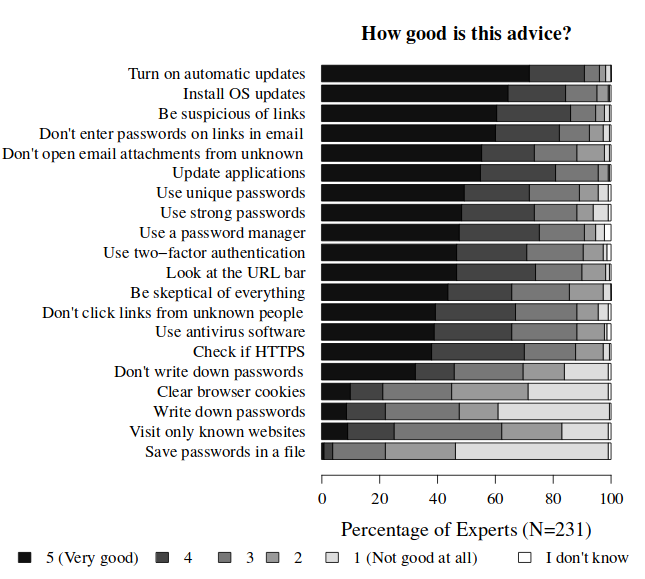
\includegraphics[width=0.7\textwidth]{figures/importance_of_updates.png}
        \caption{Sikkerhedseksperter vægter opdatering af software meget højt.\autocite{soups2015}}\label{fig:updates}
    \end{figure}
    Med IoT enheder derimod er det ikke den samme software der bliver brugt til alle enheder, og økonomisk nytter det ikke noget at blive ved med at opdatere softwaren til et 5 årt gammelt produkt, som de fleste nok allerede har skiftet ud.
    Producenter kunne i denne situation gøre det tydeligt hvornår end of life for et produkt er og hvordan de opdaterer deres software. Altså tydeliggøre hvordan man opdaterer sine IoT enheder og hvor lang tid brugeren kan forvente at være sikret. I følge sikkerhedseksperter er opdateret software er en af de absolut vigtigste elementer i et sikkert produkt. \autocite{soups2015}
    Det vil selvfølgelig ikke forhindre alle angreb fuldstændigt, men regulære sikkerhedsopdateringer gør at det blot er dem der finder, eller er er villige til at betale for \glspl{zero-day_exploit}, som vil have muligheden for at komme ind i et netværk. Uden regulære sikkerhedsopdateringer bliver disse exploits dog hurtigt offentligt tilgængelige, og kan ved en simpel søgning i en \gls{vulnerability-database} ofte findes og benyttes af en langt bredere gruppe mennesker.\\
    IoT muliggøre at mange enheder som før skulle betjenes manuelt nu kan styres via fjernadgang. For forbrugeren kan dette være en stor fordel da flere opgaver kan udføres uden man fysiks skal bevæge sig. Sikkerhedsmæssigt kan det skabe problematikker, eftersom hvor der før kun var fysisk adgang til enheden er det nu muligt at tilgå enheden fra et vilkårligt sted fra netværket eller internettet.\\ 
    Ondsindede personer kan derfor overtage produktet og misbruge informationer eller udføre fysisk skade. Fjernstyring kan være et problem men kun hvis der er huller i netværk sikkerheden og derfor vil det være bedre at fokusere på netværksikkerheden i stedet for denne problemstilling.\autocite{Forbes2017}\\
    En firewall er en barriere mellem to enheder som førhen har været fysisk da man fysisk skulle bevæge sig hen til enheden for at tilgå den. IoT bryder denne barriere ved at tillade fjernadgang sådan at man på LAN-nettet kan tilgå enheden. På et normalt hjemme LAN er der ikke nogen firewall til at styre trafikken. Det gør det nemt at kommunikere mellem enheder men sikkerhedsmæssigt er det ikke så sikkert. Den eneste firewall der så er tilbage på et LAN er den som enheden selv har men den er ofte meget åben. Grunden til denne ringe sikkerhed er at man skal være inde på LAN netværket før at man kan begynde at hacke andre hvilket førhen har været en udfordring. At komme fra internettet og ind på et LAN netværk er ikke en nem opgave da firewall'en i routeren blokere alt trafik som kommer udefra med mindre at det er noget LAN netværket specifikt har spurgt efter. Problemet opstår nu hvor IoT enheder nu også kan tilgås fra internettet så man ikke behøver at være på LAN netværket for at tilgå den. For at dette er muligt skal routeren åbne for en port så der er direkte hul fra internettet ind på LAN netværket. Det vil sige at hackere har direkte hul til at påvirke enheden så hvis enheden har en svaghed så kan den overtages. IoT enheden kan selv åbne en port i routeren uden brugeren er klar over det. Bruger enheden så stadig standard kode så er den sårbar over for angreb. Det vil derfor være en god ide at undersøge hvordan man ved hjælp af firewall kan begrænse risikoen for angreb.\\
    Det er meget relevant at se på hvordan kommunikation kan begrænses og styres på et LAN netværk da det er et område hvor der lige nu ikke er den store sikkerhed.\todo{kilde?}
    
    \subsection {Hvornår får vi nok?}
    Der er ingen tvivl om at IoT enheder kan lave vores hverdag nemmere, og effektivisere brugen af både tid og ressourcer og tid, men hvor længe vil hypen forsætte nogle IoT producenter bliver ved med at ignorere de sikkerhedsmæssige problemer som er en del af deres produkter? Er det først efter brugeren er blevet ramt at brugeren begynder at overveje hvilke producenter de vælger at købe deres produkter fra? Et eksempel på nogen der først valgte at forlade IoT muligheden efter deres IoT enheder blev brugt imod dem, kunne være et østrisk hotel som blev offer for et phsishing angreb. Her kom hackerne ind i systemet ved hjælp af et falsk link som gave hackere adgang til hotellets LAN. herfra låste hackerne hotellets IoT døre. Herefter forlangte de 2 bitcoins for at give dem kontrollen tilbage. Dette kan dog ikke kun ske for firmaer. En dag vil en hacker måske få adgang til din smart-kaffekande og kræve 30kr for at du kan få din morgenkaffe.\\
    Men for mange annoncerer hackerne ikke deres ankomst, her kommer de ind med formålet bare at indsamle data. Dette var noget man så hos et amerikansk casino som havde et akvarie som selv stod for madning, salinitet og temperatur hvilket alt sammen blev styret over LAN. Hackerne kom så ind på den måde og brugte den adgang til at stjæle 10GB værd af data. I et event som dette kan hackerne sidde på dit netværk i lang tid før du får noget at vide, hvis det altså overhovedet opdages.\autocite{Examples}
    
    
    
   
    %\subsubsection{Gammel software} Gammel version
    %Et af de store problemer ved sikkerheden i IoT enheder var den relativt korte end of life tid på meget af softwaren og firmwaren involveret. Ved end of life vil en producent typisk stoppe med at lave nye opdateringer til deres produkt, og dette inkluderer sikkerhedsopdateringer. I følge sikkerhedseksperter er opdateret software er en af de absolut vigtigste elementer i et sikkert produkt. \autocite{soups2015} Hvis software ikke bliver regelmæssigt opdateret vil den være langt mere sårbar, da den ikke vil være resistent mod de nyeste udviklinger inden for hackingangreb.
       
        
        
    %\subsection{Problemanalyse}
    %Hvad er jeres initierende undren?\\
    %Da IoT bliver sådan en stor del af vores hverdag vil vi gerne kende de problemer der kan opstå. \\
    
    


    
    %\subsection{Problemtyper} %Måske skal det slettes
    %Anomali\\ \todo{Skal vist bare slettes}
    %Et sikkerhedhul er en anomali\\
    %Paradoks\\
    %Beslutningsproblemer\\
    %Normalier\\
    %At der er huller som er accepteret er normalier\\
